\section{Reflectors}

The material of choice for the KDBs (Kapton) as many advantages including flexibility, little degassing and radiopurity. However it is a poor reflector. In order to increase the amount of light recorded by the energy plane, a 2 mm teflon reflector is placed in front of each KDB. The reflectors (Fig. \ref{fig:reflector}) have holes to accommodate the SiPMs without damaging them and also have a space for the thermal sensor and the LEDs. However no holes are neccesary for the LEDs, since teflon is sufficiently transparent to the blue light they emit. 
\begin{figure}[h!]
\centering
\includegraphics[width=0.45\textwidth]{IMG/teflon1}
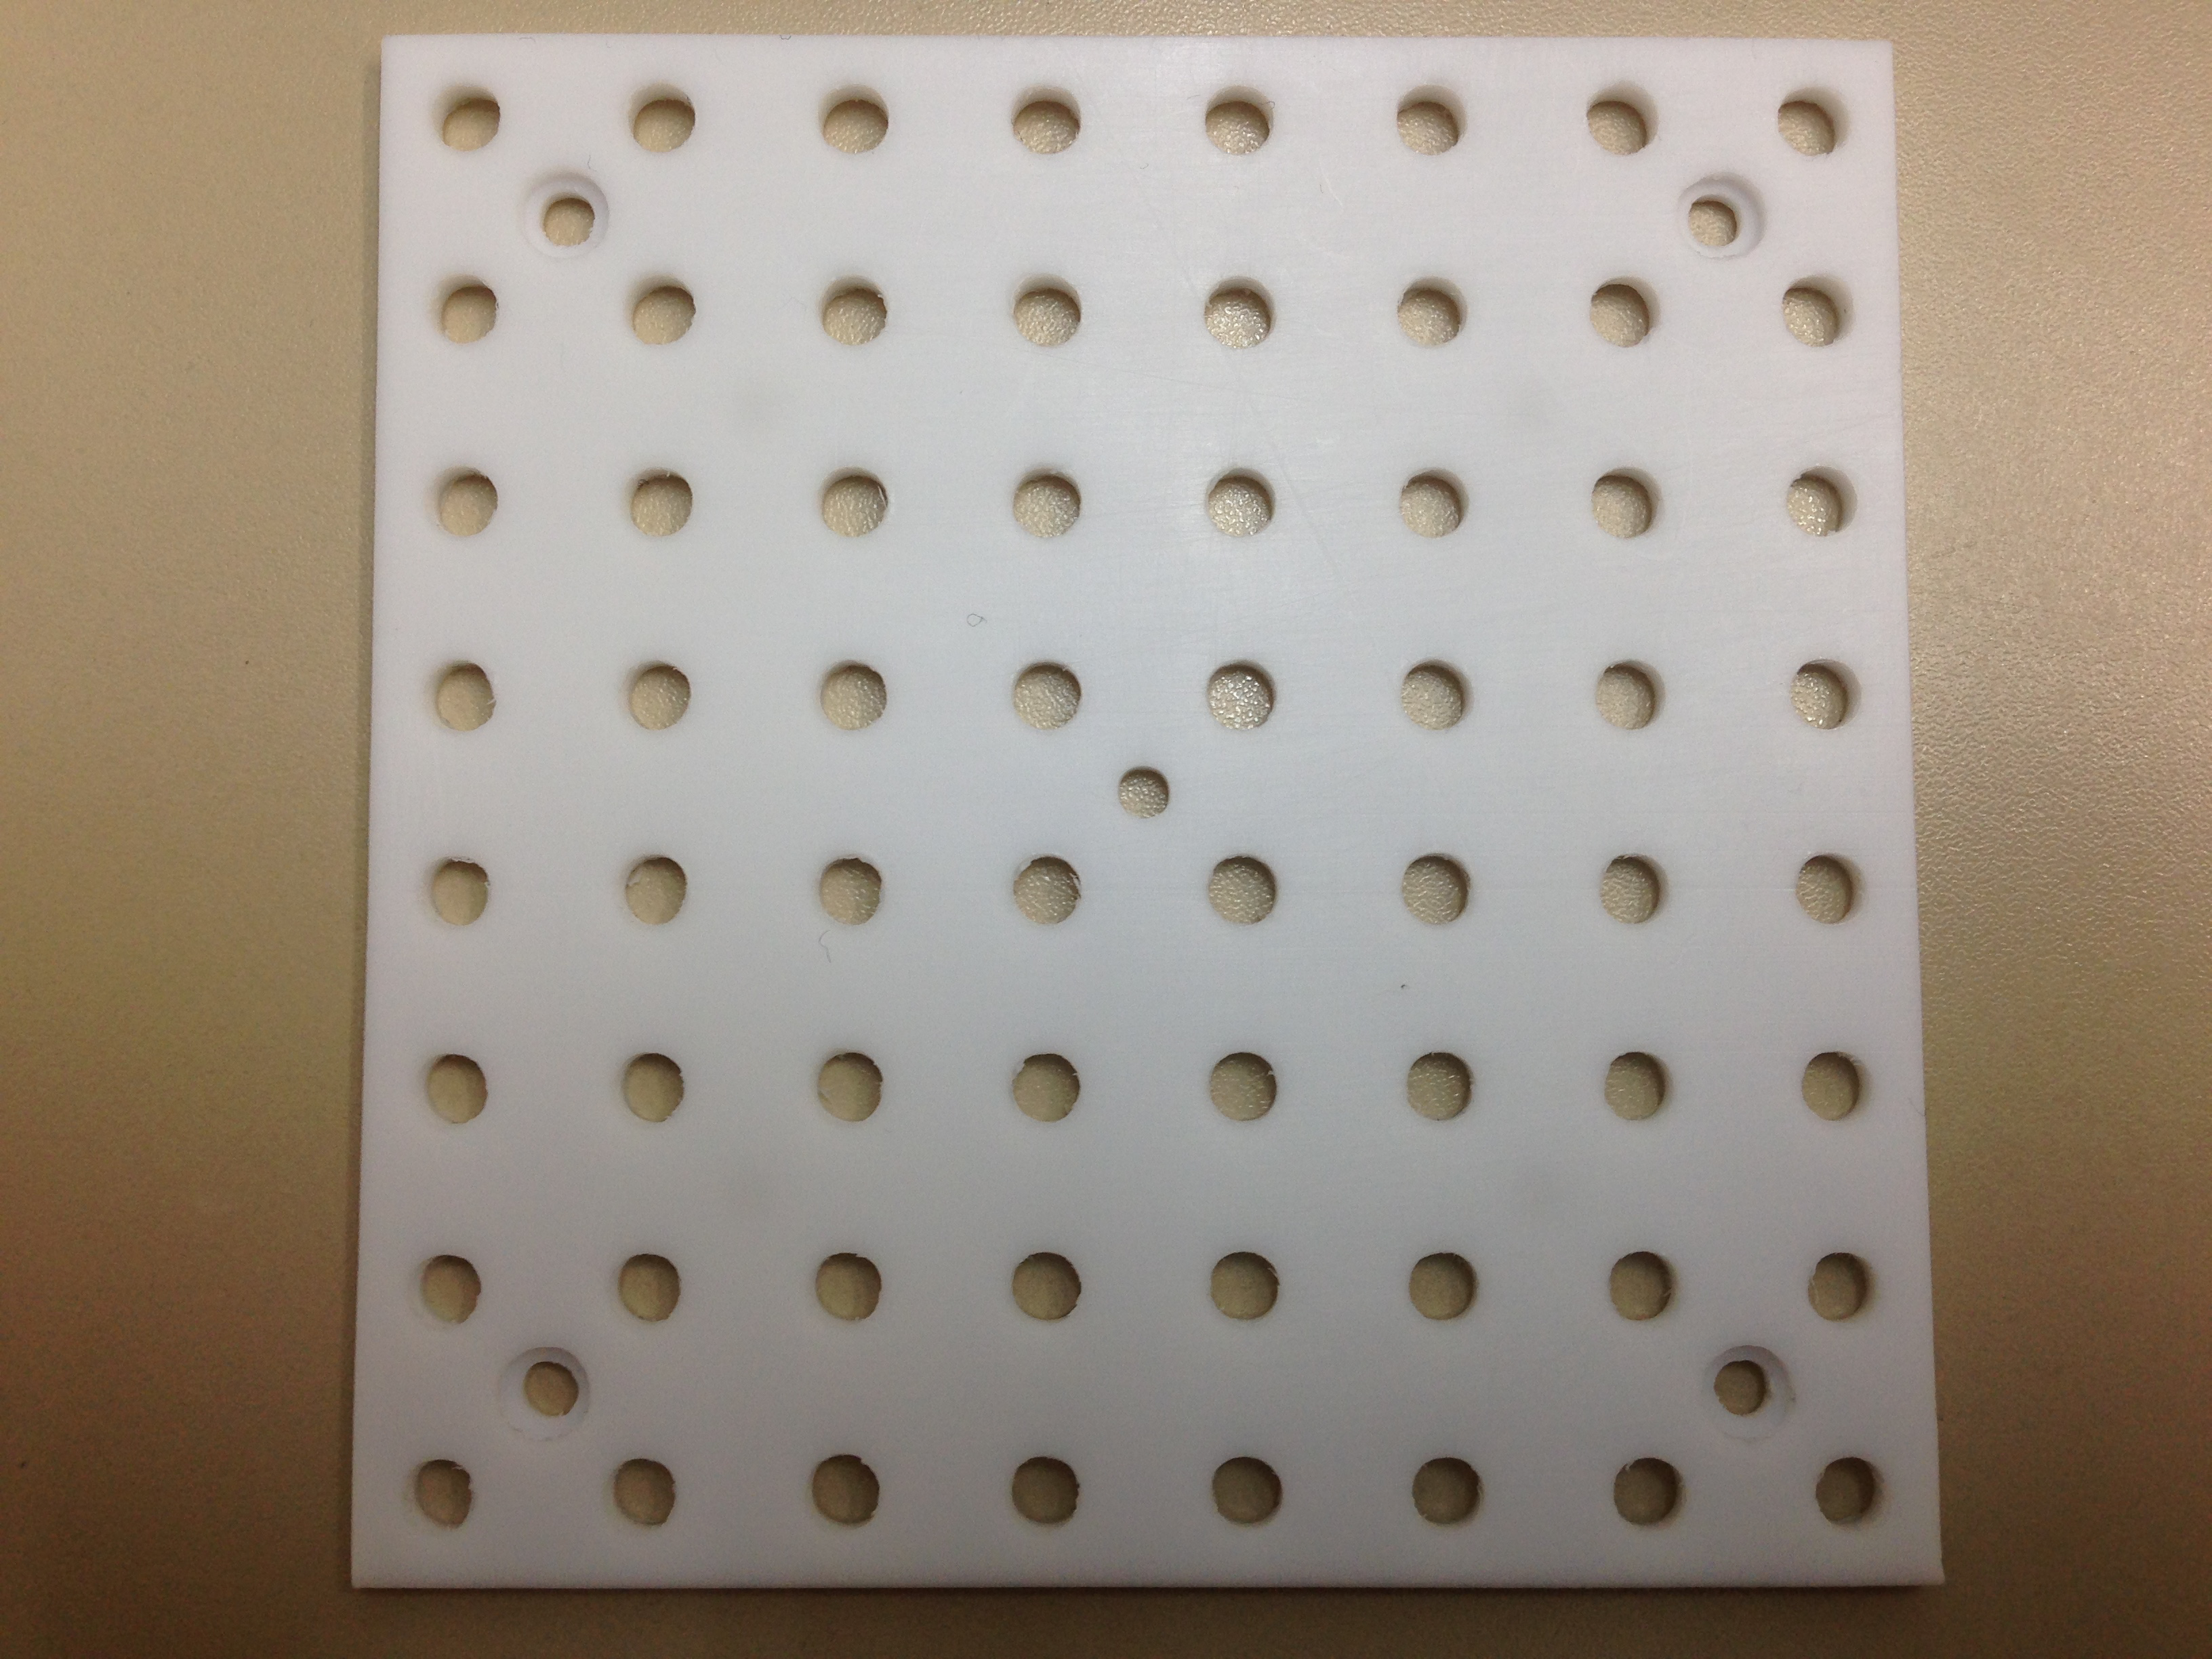
\includegraphics[width=0.45\textwidth]{IMG/teflon2}
\caption{Left: Back side (DB side) of the reflector. Right: Front side (EL) of the reflector.}
\label{fig:reflector}
\end{figure}

